
The main purpose of this lab activity is to get familiarized with the gas proportional chamber detector. For that a two gas chamber detectors were built 
from scratch using the simple components and relatively easy available parts. One of the detectors was built by using a piece of Al tube and the other by using a common beer can. 
For both detectors the spectrum of radioactive sources Fe-55 and Am-241 were measured. 

\begin{figure}[!h]
  \centering
  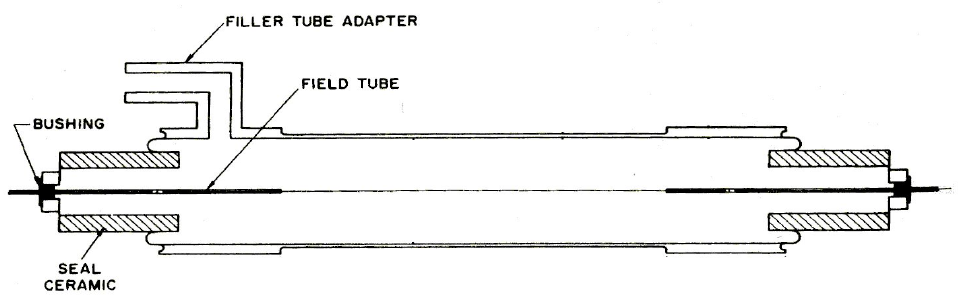
\includegraphics[width=.5\linewidth]{prop_counter_cross_section}
  \caption{Cross sectional view of the proportional counter\autocite{Knoll:RadMeasurement}.}
  \label{fig:prop_count_cs}
\end{figure}
Insert introduction
%%% Local Variables:
%%% mode: latex
%%% TeX-master: "prop_counter"
%%% End:
